\documentclass[../main.tex]{subfiles}

\begin{document}
    \section{Vector Fields and the Tangent Bundle}
    \subsection{Vector Fields}
    \begin{definition}[Vector Fields]\label{def:vector-fields}
        A vector field \(X\) on \(V \subseteq\manifold[M]\) is any rule of assigning 
        a tangent vector \(X(p) = X_p \in T_p\manifold[M]\) for all
        \(p \in V\).
    \end{definition}
    \begin{definition}[Components of a Vector Field]\label{def:vector-field-component}
        Let \(X\) be a vector field on \(V \subseteq \manifold[M]\), 
        \(\dim \manifold[M] = m\). For any chart \(\phi : U \to \phi(U) \in \Phi\) 
        with induced coordinates \(x^1, \dots, x^m\) and any \(p \in V \cap U\), 
        the decomposition \(X(p) = X^j(p)\tvec{j}{p}\) is unique, and therefore 
        we write 
        \[
        X = X^j \tfld{j}
        \]
        on \(V \cap U\), and \(X^j : V \cap U \to \mathbb{R}\) are called the 
        components of \(X\) on \(V \cap U\).
    \end{definition}
    \begin{definition}[Smoothness of a Vector Field]\label{def:vec-field-smoothness}
        A vector field \(X\) on \(V \subseteq \manifold[M]\) is \(C^k\) near 
        \(p \in V\) iff \(\exists~\phi \in \Phi\) s.t. \(p \in U_\phi\) and all 
        the components \(X^j\) induced by \(\phi\) are \(C^k\). That is, 
        \[
        X^j\circ \phi ^{-1} \text{ are } C^k \text{ on } \phi(V \cap U).
        \]
    \end{definition}

    \subsection{Tangent Bundle}
    \subsubsection{Definition}
    \begin{definition}[Tangent Bundle]\label{def:tangent-bundle}
        The tangent bundle \(T\manifold[M]\) is 
        \[
        T\manifold[M] := \bigcup_{p \in \manifold[M]}^{} T_p\manifold[M].
        \]
    \end{definition}
    \begin{remark}
        Why not \(T\manifold[M] := \Set{T_p\manifold[M]|p \in \manifold[M]}\)?
    \end{remark}
    \subsubsection{Projection}
    \begin{definition}[Canonical Projection]\label{def:canonical-projection}
        The canonical projection is the map 
        \[
        \begin{aligned}
            \pi : T\manifold[M] &\to \manifold[M] \\
            T_p\manifold[M] &\mapsto p.
        \end{aligned}
        \]
    \end{definition}
    \begin{definition}[Alternative Definition of Vector Fields]\label{def:vector-fields-alt}
        A tangent vector field \(X\) on \(V \subseteq \manifold[M]\) is a map 
        \(X : V \to T\manifold[M]\) s.t. \((\pi \circ X)(p) = p\) for all \(p \in V\).
    \end{definition}
    \begin{remark}
        Let's see why vector fields are often called a "cross-section" of a tangent 
        bundle.
        \begin{center}
            \includegraphics{./figs/bundle.pdf}
        \end{center}
    \end{remark}
    \newpage
    \subsubsection{Topological and Manifold Structure}
    \begin{definition}[Smooth Structure on Tangent Bundle]\label{def:smooth-structure-tangent-bundle}
        Let a manifold \(\manifold[M]\) with dimension \(m\) and atlas \(\Phi\). 
        Consider a chart \(\phi_j \in \Phi : U_j \to \mathbb{R}^m\). We define 
        a chart \(\tilde{\phi}_j\) for the tangent bundle \(T\manifold[M]\) 
        accordingly, 
        \[
        \begin{aligned}
            \tilde{\phi}_j : \tilde{\pi}(U_j) \subseteq T\manifold[M] &\to 
            \mathbb{R}^{2m} \\
            (p, v^i\tfld{i}) &\mapsto (\phi_j(p), v^1, \dots, v^m),
        \end{aligned}
        \]
        where \(\tilde{\pi}\) is the inverse set map of the canonical projection 
        function \cref{def:canonical-projection}. We thus see the tangent bundle 
        \(T\manifold[M]\) is itself a manifold of dimension \(2m\).\\
        Also, we define the topology of the tangent bundle by 
        \[
        A \subseteq T\manifold[M] \text{ is open iff }
        \tilde{\phi}_j(A \cap \tilde{\pi}(U_j)) \text{ is open.}
        \]
    \end{definition}
    \begin{theorem}
        The smooth structure given by \cref{def:smooth-structure-tangent-bundle} 
        is unique in the sense of, 
        \begin{enumerate}
            \item \(\pi : T\manifold[M] \to \manifold[M]\) is \(C^\infty\),
            \item For all open sets \(V \subseteq \manifold[M]\) and any vector 
            field \(X\) on \(V\), \(X \text{ is } C^\infty \iff 
            X : V \to T\manifold[M]\) is \(C^\infty\).
        \end{enumerate}
    \end{theorem}
    \begin{remark}
        At first thought, one may think of \(T\manifold[M] \iso 
        \manifold[M] \times \mathbb{R}^m\). This is not the case, as one can 
        consider the Moebius strip. The tangent bundle is only locally 
        isomorphic to \(U \times \mathbb{R}^m\).\\
        If indeed \(T\manifold[M] \simeq \manifold[M] \times \mathbb{R}^m\), 
        then the bundle is called trivial tangent bundle, and the manifold is 
        called parallelizable.
    \end{remark}

    \newpage
    \subsection{Integral Curves and Local Flows}
    \subsubsection{Integral Curves}
    \begin{definition}[Integral Curves]\label{def:integral-curve}
        Let \(\manifold[M]\) be a manifold, and \(X\) be a vector field on 
        \(V \subseteq \manifold[M]\).
        If one single curve \(\sigma : (-\epsilon, \epsilon) \to V\), 
        \(\epsilon > 0\) satisfies 
        \[
        \begin{aligned}
            \sigma(0) &= p \in V \\
            X_{\sigma(t)} &= [\sigma]\; \forall t \in (-\epsilon, \epsilon)
        \end{aligned}
        \]
        then \(\sigma\) is called an integral curve of the vector field \(X\) 
        through the point \(p\).
    \end{definition}
    \begin{theorem}[Differential Equations of Integral Curve]\label{thm:de-int-curve}
        The components \(X^\mu\) of \(X\) determine the integral curve \(\sigma\) 
        by the following ODE with boundary conditions, 
        \[
        \begin{aligned}
            X^\mu(\sigma(t)) &= \frac{d}{dt}x^\mu(\sigma(t)) \\
            x^\mu(\sigma(0)) &= x^\mu(p), \mu = 1, 2, \dots, m.
        \end{aligned}
        \]
    \end{theorem}
    \subsubsection{Local Flows}
    \begin{definition}[Local 1D Family of Local Diffeomorphisms]\label{def:local-diff}
        A local, 1D family of local diffeomorphisms at \(p \in \manifold[M]\) 
        is made up of a family of diffeomorphisms \(\Set{\sigma_t : U \to 
        \manifold[M]|t \in (-\epsilon, \epsilon)}\) with \(\epsilon > 0\), 
        \(U \subseteq \manifold[M]\) an open set s.t. 
        \begin{enumerate}
            \item Every \(\sigma_t\) is a smooth function in \(t\) and \(p\).
            \item \(\forall t, s \in \mathbb{R}\) and \(|t|, |s|, |t+s| < 
            \epsilon\), and \(\forall p \in U\) s.t. \(\sigma_t(p), \sigma_s(p), 
            \sigma_{t+s}(p) \in U\), we have 
            \[
            \sigma_s(\sigma_t(p)) = \sigma_{s+t}(p).
            \]
            \item \(\sigma_0(p)=p\).
        \end{enumerate}
    \end{definition}
    \begin{remark}
        The first "local" refers to the parameter \(t\), which is limited to 
        \((-\epsilon, \epsilon)\). The second "local" refers to the spatial 
        limitation to \(U\). 
        You can view \(\phi_t(q)\) as a curve that brings \(t \in (-\epsilon, 
        \epsilon)\) to \(\phi_t(q) \in \manifold[M]\).
    \end{remark}
    \begin{definition}
        Consider a family of local diffeomorphisms given by \cref{def:local-diff} 
        \(\phi_t\). We denote the following for convenience, if its meaning is 
        clear from context, 
        \[
        \begin{aligned}
            \sigma(p, t) &:= \sigma_t(p), \\
            \sigma_p(t)  &:= \sigma_t(p).
        \end{aligned}
        \]
    \end{definition}
    \begin{definition}[Local Flow]\label{def:local-flow}
        Let \(X\) be a vector field on \(V \subseteq \manifold[M]\), \(p \in V\). 
        Consider a family of diffeomorphisms \cref{def:local-diff} \(\sigma\) on 
        \(V\).
        Let the corresponding curve family \(\sigma_p(t)\) satisfy, 
        \[
        \begin{aligned}
            \sigma_p(0) &= p & &\forall p \in V, \\
            [\sigma_p] &= X_{\sigma_p(t)} = \sigma_{p*}\left(\frac{d}{dt}\right)_t
            & &\forall t \in (-\epsilon, \epsilon), p \in V.
        \end{aligned}
        \]
        Then we say the curve family \(\sigma_p(t)\) is the local flow for \(X\) 
        on \(V\).
        We may abbreviate and just say \(\sigma\) is the local flow for \(X\).
    \end{definition}
    \begin{theorem}
        Local flows always exist and are unique. Thus for a vector field \(X\) 
        defined on \(V\), we may denote its local flow of over an open set \(U\) 
        by \(\sigma^X\).
    \end{theorem}
    % \begin{definition}[Induced Vector Field]\label{def:induced-vector-field}
    %     By taking tangents to the curve family \cref{def:local-diff}, we have 
    %     the induced vector field \(X^\phi\) given by
    %     \[
    %     X^\phi_q(f) := \left.\frac{d}{dt}(f(\phi_t(q)))\right|_{t=0}
    %     \]
    % \end{definition}
    % \begin{theorem}
    %     The curve family \(t \mapsto \phi_t(q)\) is the integral curve of 
    %     the induced vector field \cref{def:induced-vector-field} \(X^\phi_q\).
    % \end{theorem}
    % \begin{proof}
    %     \[
    %     \begin{aligned}
    %         X^\phi_{\phi_s(q)} &= \left.\frac{d}{dt}
    %         (f\circ\phi_t\circ\phi_s(q))\right|_{t=0} \\
    %         &= \left.\frac{d}{dt}(f\circ\phi_{t+s}(q))\right|_{t=0}.
    %     \end{aligned}
    %     \]
    %     Let \(u = t+s\). Then 
    %     \[
    %     \begin{aligned}
    %         X^\phi_{\phi_s(q)} &= 
    %         \left.\frac{d}{du}(f\circ\phi_{u}(q))\right|_{u=s}. \\
    %         &= \phi_{q*}\left(\frac{d}{dt}\right)_sf.
    %     \end{aligned}
    %     \]
    % \end{proof}

    \newpage
    \subsection{Lie Derivative of Vector Fields}
    \subsubsection{Lie Bracket}
    \begin{definition}[Lie Derivative of Functions]\label{def:lie-der-function}
        We can view a vector field as a function \(X : C^\infty \to C^\infty\), 
        given by
        \[
        (Xf)(p) := X_pf = \left.\frac{\partial }{\partial t}
        (f\circ \sigma^X(p, t))\right|_{t=0}.
        \]
        We can interpret this as: How much the function \(f\) changes beginning 
        at \(p\), along the flow lines of \(X\)?
    \end{definition}
    \begin{definition}[Composition of Vector Fields]\label{def:vector-field-composition}
        We can view \(X : C^\infty(\manifold[M]) \to C^\infty(\manifold[M])\), 
        and so does \(Y\). Therefore, we define 
        \[
        (X \circ Y)(f) := X(Yf).
        \]
    \end{definition}
    \begin{theorem}[Flow Interpretation]\label{thm:vector-field-composition-flow}
        \[
        X_p(Yf) = \left.\frac{\partial ^2}{\partial s\partial t}\left(
            f \left(\sigma^Y \left(\sigma^X(p, t), s\right)\right)
        \right)\right|_{(s, t)=(0, 0)}.
        \]
        We can interpret \(X(Yf)\) as: How much the function \(f\) changes 
        beginning at the point \(p\), first following the flow lines of \(X\), 
        then following the flow lines of \(Y\)?
    \end{theorem}
    \begin{definition}[Lie Bracket/Vector Field Commutator]\label{def:lie-bracket}
        We define the Lie Bracket of two vector fields \(X, Y\) to be 
        \[
        [X, Y] := X\circ Y - Y\circ X.
        \]
    \end{definition}
    \begin{remark}
        Lie Bracket \cref{def:lie-bracket} is a vector field, while the 
        expression \(X\circ Y\) is not, because it contains second differential 
        terms. See the following proof.
    \end{remark}
    \begin{theorem}[Lie Bracket Components]\label{thm:lie-bracket-components}
        \[
        [X, Y]^\mu = (X^\nu\tfld{\nu}Y^\mu - Y^\nu\tfld{\nu}X^\mu).
        \]
    \end{theorem}
    \begin{proof}
        Given \(X=X^\mu\tfld{\mu}, Y = Y^\nu\tfld{\nu}\), we try to write 
        the component of \(X\circ Y\).
        \[
        X\circ Y(f) = X^\mu \tfld{\mu}\left(Y^\nu \tfld{\nu}f\right).
        \]
        However, notice that 
        \[
        \begin{aligned}
            &Y^\nu := Yx^\nu \in C^\infty(\manifold[M]); \\
            &\tfld{\nu} : C^\infty(\manifold[M]) \to C^\infty(\manifold[M]), \\
            &\implies\tfld{\nu}f \in C^\infty(\manifold[M]).
        \end{aligned}
        \]
        So we need to use the Leibniz property of \(\tfld{\mu}\) 
        in order to evaluate the second term. Doing this 
        for \(X\circ Y(f)\) and \(Y\circ X(f)\), we have
        \[
        \begin{aligned}
            X\circ Y(f) &= X^\mu \left((\tfld{\mu}Y^\nu)(\tfld{\nu}f)+
            Y^\nu \tfld{\mu}\tfld{\nu}f\right). \\
            Y\circ X(f) &= Y^\nu \left((\tfld{\nu}X^\mu)(\tfld{\mu}f)+
            X^\mu \tfld{\nu}\tfld{\mu}f\right).
        \end{aligned}
        \]
        So if \(\tfld{\mu}\tfld{\nu}f=\tfld{\nu}\tfld{\mu}f\), then by 
        subtracting, we can cancel the second order terms, and we are done. We 
        prove so now.
        \[
        \begin{aligned}
            (\tfld{\mu}\tfld{\nu}f)(p)&=\left.\frac{\partial }{\partial u^\mu}
            \left((\tfld{\nu}f)\circ\phi ^{-1}\right)\right|_{\phi(p)} \\
            &=\left.\frac{\partial }{\partial u^\mu}
            \left(\tvec{\nu}{\phi ^{-1}(u)}f\right)\right|_{\phi(p)} \\
            &=\left.\frac{\partial }{\partial u^\mu}
            \left(\left.
                \frac{\partial }{\partial u^\nu}(f\circ\phi ^{-1})
            \right|_u\right)\right|_{\phi(p)} \\
            &=\left.\frac{\partial }{\partial u^\nu}
            \left(\left.
                \frac{\partial }{\partial u^\mu}(f\circ\phi ^{-1})
            \right|_u\right)\right|_{\phi(p)} \\
            &=(\tfld{\nu}\tfld{\mu}f)(p).
        \end{aligned}
        \]
    \end{proof}
    \newpage
    \begin{theorem}[Properties of Lie Brackets]\label{thm:lie-bracket-properties}
        \[
        \begin{cases}
            [X,Y] = -[Y, X] & \text{(antisymmetry)} \\
            \sum_{\text{cyc}}^{} [X, [Y, Z]]=0. & \text{(Jacobi Identity)}
        \end{cases}
        \]
    \end{theorem}

    \subsubsection{Lie Derivative of Vector Fields}
    \begin{definition}[Lie Derivative]\label{def:lie-derivative}
        Let \(X, Y\) be two vector fields defined on \(U, V \subseteq 
        \manifold[M]\), respectively. Then the lie derivative of \(Y\) 
        along \(X\) is defined as 
        \[
        (\lder{X}Y)_p := 
        \lim_{t \to 0} \frac{\sigma^X_{-t*}(Y_{\sigma^X_t(p)}) - Y_p}{t},
        \]
        where the latter is often abbreviated as 
        \[
        \left.\frac{d}{dt}(\sigma_{-t*}^X(Y_{\sigma^X_t(p)}))\right|_{t=0}=
        \lim_{t \to 0} \frac{\sigma^X_{-t*}(Y_{\sigma^X_t(p)}) - Y_p}{t}.
        \]
    \end{definition}
    \begin{remark}
        It is common to interpret the Lie derivative of \(Y\) along \(X\) to 
        be: How much do \(Y\) change when one moves along the flow lines of 
        \(X\)? \\
        However, one cannot directly compare the two vectors \(Y_{\sigma^X_t(p)}
        \in T_{\sigma^X_t(p)}\manifold[M]\) and \(Y_p \in T_p\manifold[M]\). 
        Therefore, the most intuitive way is to "pull it back", i.e., push it 
        forward along the flow lines of \(X\) by negative time.
    \end{remark}
    \begin{theorem}[Lie Bracket and Lie Derivative]\label{thm:lie-bracket-flow}
        \[
        \lder{X}Y = [X, Y].
        \]
        That is, 
        \[
        \left.\frac{d}{dt}(\sigma_{-t*}^X(Y_{\sigma^X_t(p)}))\right|_{t=0}
        = X\circ Y - Y \circ X.
        \]
    \end{theorem}
    \begin{proof}
        We start with 
        \[
        \begin{aligned}
            \left.\frac{d}{dt}(\sigma_{-t*}^X(Y_{\sigma^X_t(p)}))\right|_{t=0}f
            &=\lim_{t \to 0} \frac{\sigma^X_{-t*}(Y_{\sigma^X_t(p)f}) - Y_pf}{t} \\
            &=\lim_{t \to 0} \frac{Y_{\sigma^X_t(p)}(f\circ\sigma^X_{-t}) - 
            Y_{\sigma^X_0(p)}(f\circ \sigma^X_0)}{t}.
        \end{aligned}
        \]
        It motivates us to consider the function 
        \(H(r, s) = Y_{\sigma^X_r(p)}(f\circ\sigma^X_{-s})\).
        Then we see 
        \[
        \begin{aligned}
            \left.\frac{d}{dt}(\sigma_{-t*}^X(Y_{\sigma^X_t(p)}))\right|_{t=0}f
            &= \left.\frac{d}{dt}H(t, t)\right|_{t=0} \\
            &=\frac{\partial H}{\partial r}(0, 0) + 
            \frac{\partial H}{\partial s}(0, 0).
        \end{aligned}
        \]
        \par
        (\(r\) part: moving along \(X\))
        \[
        \begin{aligned}
            \frac{\partial H}{\partial r}(0, 0)
            &=\left.\frac{\partial }{\partial r}
            Y_{\sigma^X_r(p)}(f\circ \underbrace{\sigma^X_0}_{\idd})\right|_{r=0} \\
            &=\left.\frac{\partial }{\partial r}
            (Yf)(\sigma^X_r(p))\right|_{r=0} \\
            &=X_p(Yf).
        \end{aligned}
        \]
        \par
        (\(s\) part: moving along \(Y\))
        \[
        \begin{aligned}
            \frac{\partial H}{\partial s}(0, 0)
            &=\left.\frac{\partial }{\partial s}
            Y_{p}(f\circ \sigma^X_{-s})\right|_{s=0} \\
            &=Y_{p}\left.\frac{\partial }{\partial s}
            (f\circ \sigma^X_{-s})\right|_{s=0} \\
            &=-Y_p(Xf),
        \end{aligned}
        \]
        and therefore completes the proof.
    \end{proof}
\end{document}